% !TEX root = ../masterthesis.tex
\chapter{Scanning Fabry-Pérot Interferometer}

\section{Motivation}

Resolve QD emission line.

\section{Theory}

\subsection{Gaussian Beam}

Dot-Spectra in far field is (TEM$_{00}$).

\subsection{Fabry-Pérot Interferometer}

The Fabry-Pérot interferometer is an optical resonator developed by Charles Fabry and Alfred Pérot.
An incoming light beam will only be transmitted through the resonator consisting of two semi-transparent mirrors if it fulfils the resonance condition.\cite{kaldewey_coherent_2017}

\subsection{Resonator losses an outcoupled light}
For the following discussion of the Fabry-Pérot interferometer, a two-mirror-resonator with the reflecting surfaces facing each other and air as medium in between is assumed. The time the light needs for one roundtrip is then given by ~\cite{ismail_fabry-perot_2016}
\begin{equation}
t_{RT} = \frac{2l}{c}
\end{equation}
where $l$ is the geometrical length of the resonator and $c$ is the speed of light in air. 

The photon-decay time $\tau_c{\nu}$ of the interferometer is then given by
\begin{equation}
\frac{1}{\tau_c} = - \frac{\ln(R_1 \cdot R_2)}{t_{RT}}
\end{equation}
where $R_1$ and $R_2$ are the corresponding intensity reflectivities of the mirrors.

The number of photons at frequency $\nu$ inside the resonator is described by the differential rate equation
\begin{equation}
\frac{d}{dt} \varphi(t) = - \frac{1}{\tau_c}\varphi(t)
\end{equation}
With a number $\varphi_s$ of photons at $t=$ the integration gives
\begin{equation}
\varphi(t)=\varphi_s e^{-t/\tau_c}
\end{equation}

\subsection{Airy distribution of the Fabry-Pérot interferometer}

\subsection{Simulation}

\begin{figure}[H]
	\centering
	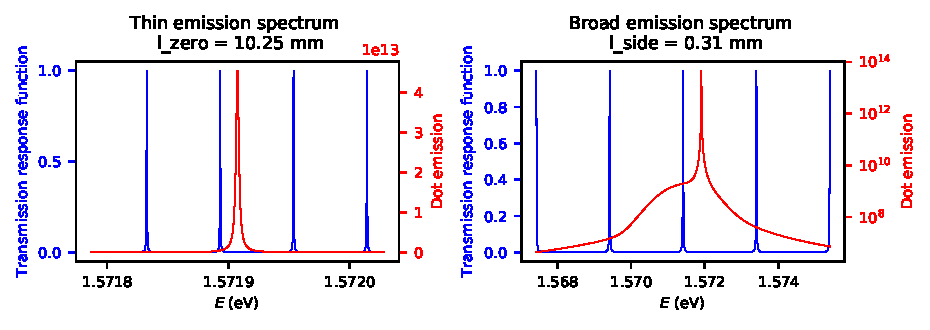
\includegraphics[width=\linewidth]{figures/plots/fabry-perot/simulation-comparison-dot-fabry-perot-modes}
	\caption{}
	\label{fig:simulation-comparison-dot-fabry-perot-modes}
\end{figure}

\section{Setup}

\subsection{Flat mirrors}


\subsection{Concave mirrors}

\subsection{Confocal setup}

\section{Measurements and Results}

